\documentclass[10pt,a4paper]{article}
	\usepackage[utf8]{inputenc} %caractères européens de l'ouest
		\usepackage[T1]{fontenc}
		%\usepackage [frenchb]{babel}%pour suivre les règles de la langue française
\usepackage{chronosys}
\begin{document}


1) Résultats préliminaires:\\

Après nous être penché sur l'état de l'art de notre sujet, nous nous sommes concertés avec notre tuteur pour définir la feuille de route de notre projet, dont les échéances sont décrites plus bas. 

A ce jour, nous avons commencé la première partie du projet, qui consiste en la réalisation d'une interface graphique à but pédagogique permettant aux élèves de se familiariser avec les concepts de base de la théorie du portefeuille optimal de Markovitz.

Une première équipe se charge de la réalisation de l'interface graphique, une autre équipe est chargée d'implémenter algorithmiquement la recherche du portefeuille de Markovitz et une troisième équipe s'occupe de la simulation des données dont on a besoin. 

2) Echéancier:\\
\begin{enumerate}
\item Début Octobre: interface graphique prête à être utilisée.
\item Avant le 1er Novembre: premières expériences réalisées avec des élèves, avec les données que nous avons générées. 
\item Avant la fin de l'année: étude de la validité de la théorie avec des données réelles (données de marché).
\item Avant la fin de l'année: expériences sur la perception visuelle des corrélations.
\item Avant mars 2019: interprétation des résultats et conclusion. 

\end{enumerate}

\begin{figure}[h!]
\centerline{
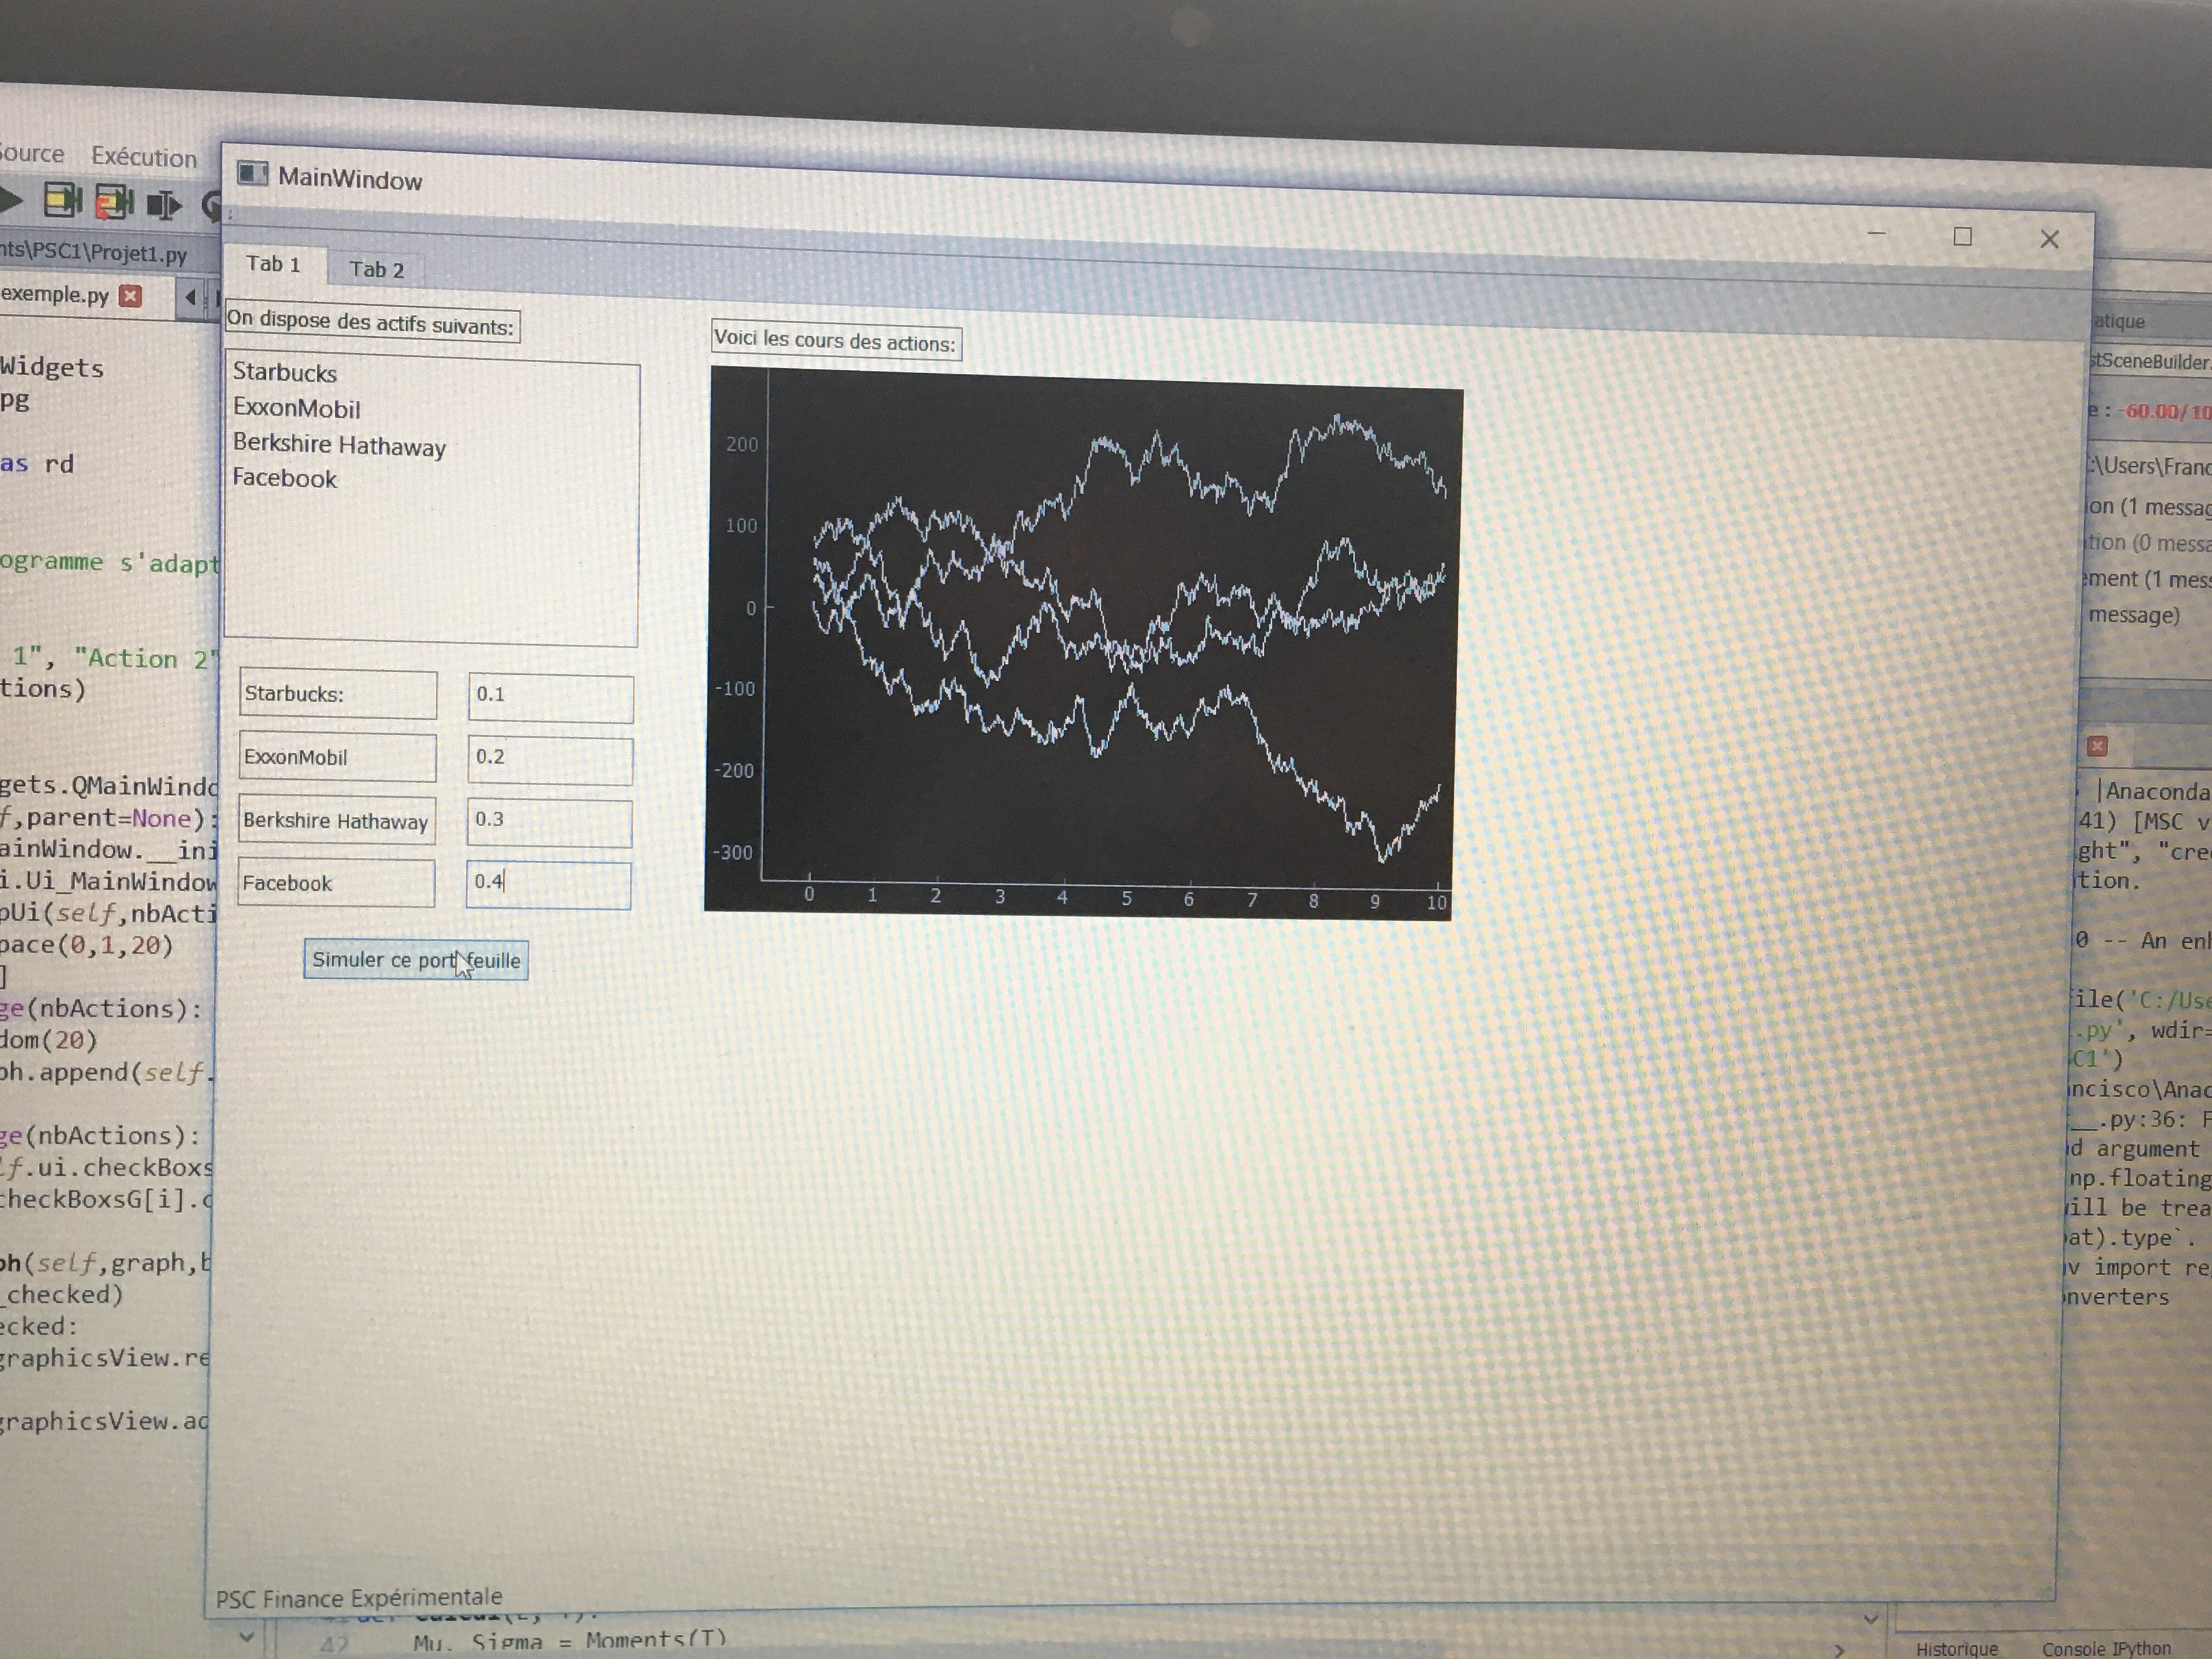
\includegraphics [width=8cm]{Im1.PNG}}
\caption{\label{} Cours des actions}
\end{figure} 

\begin{figure}[h!]
\centerline{
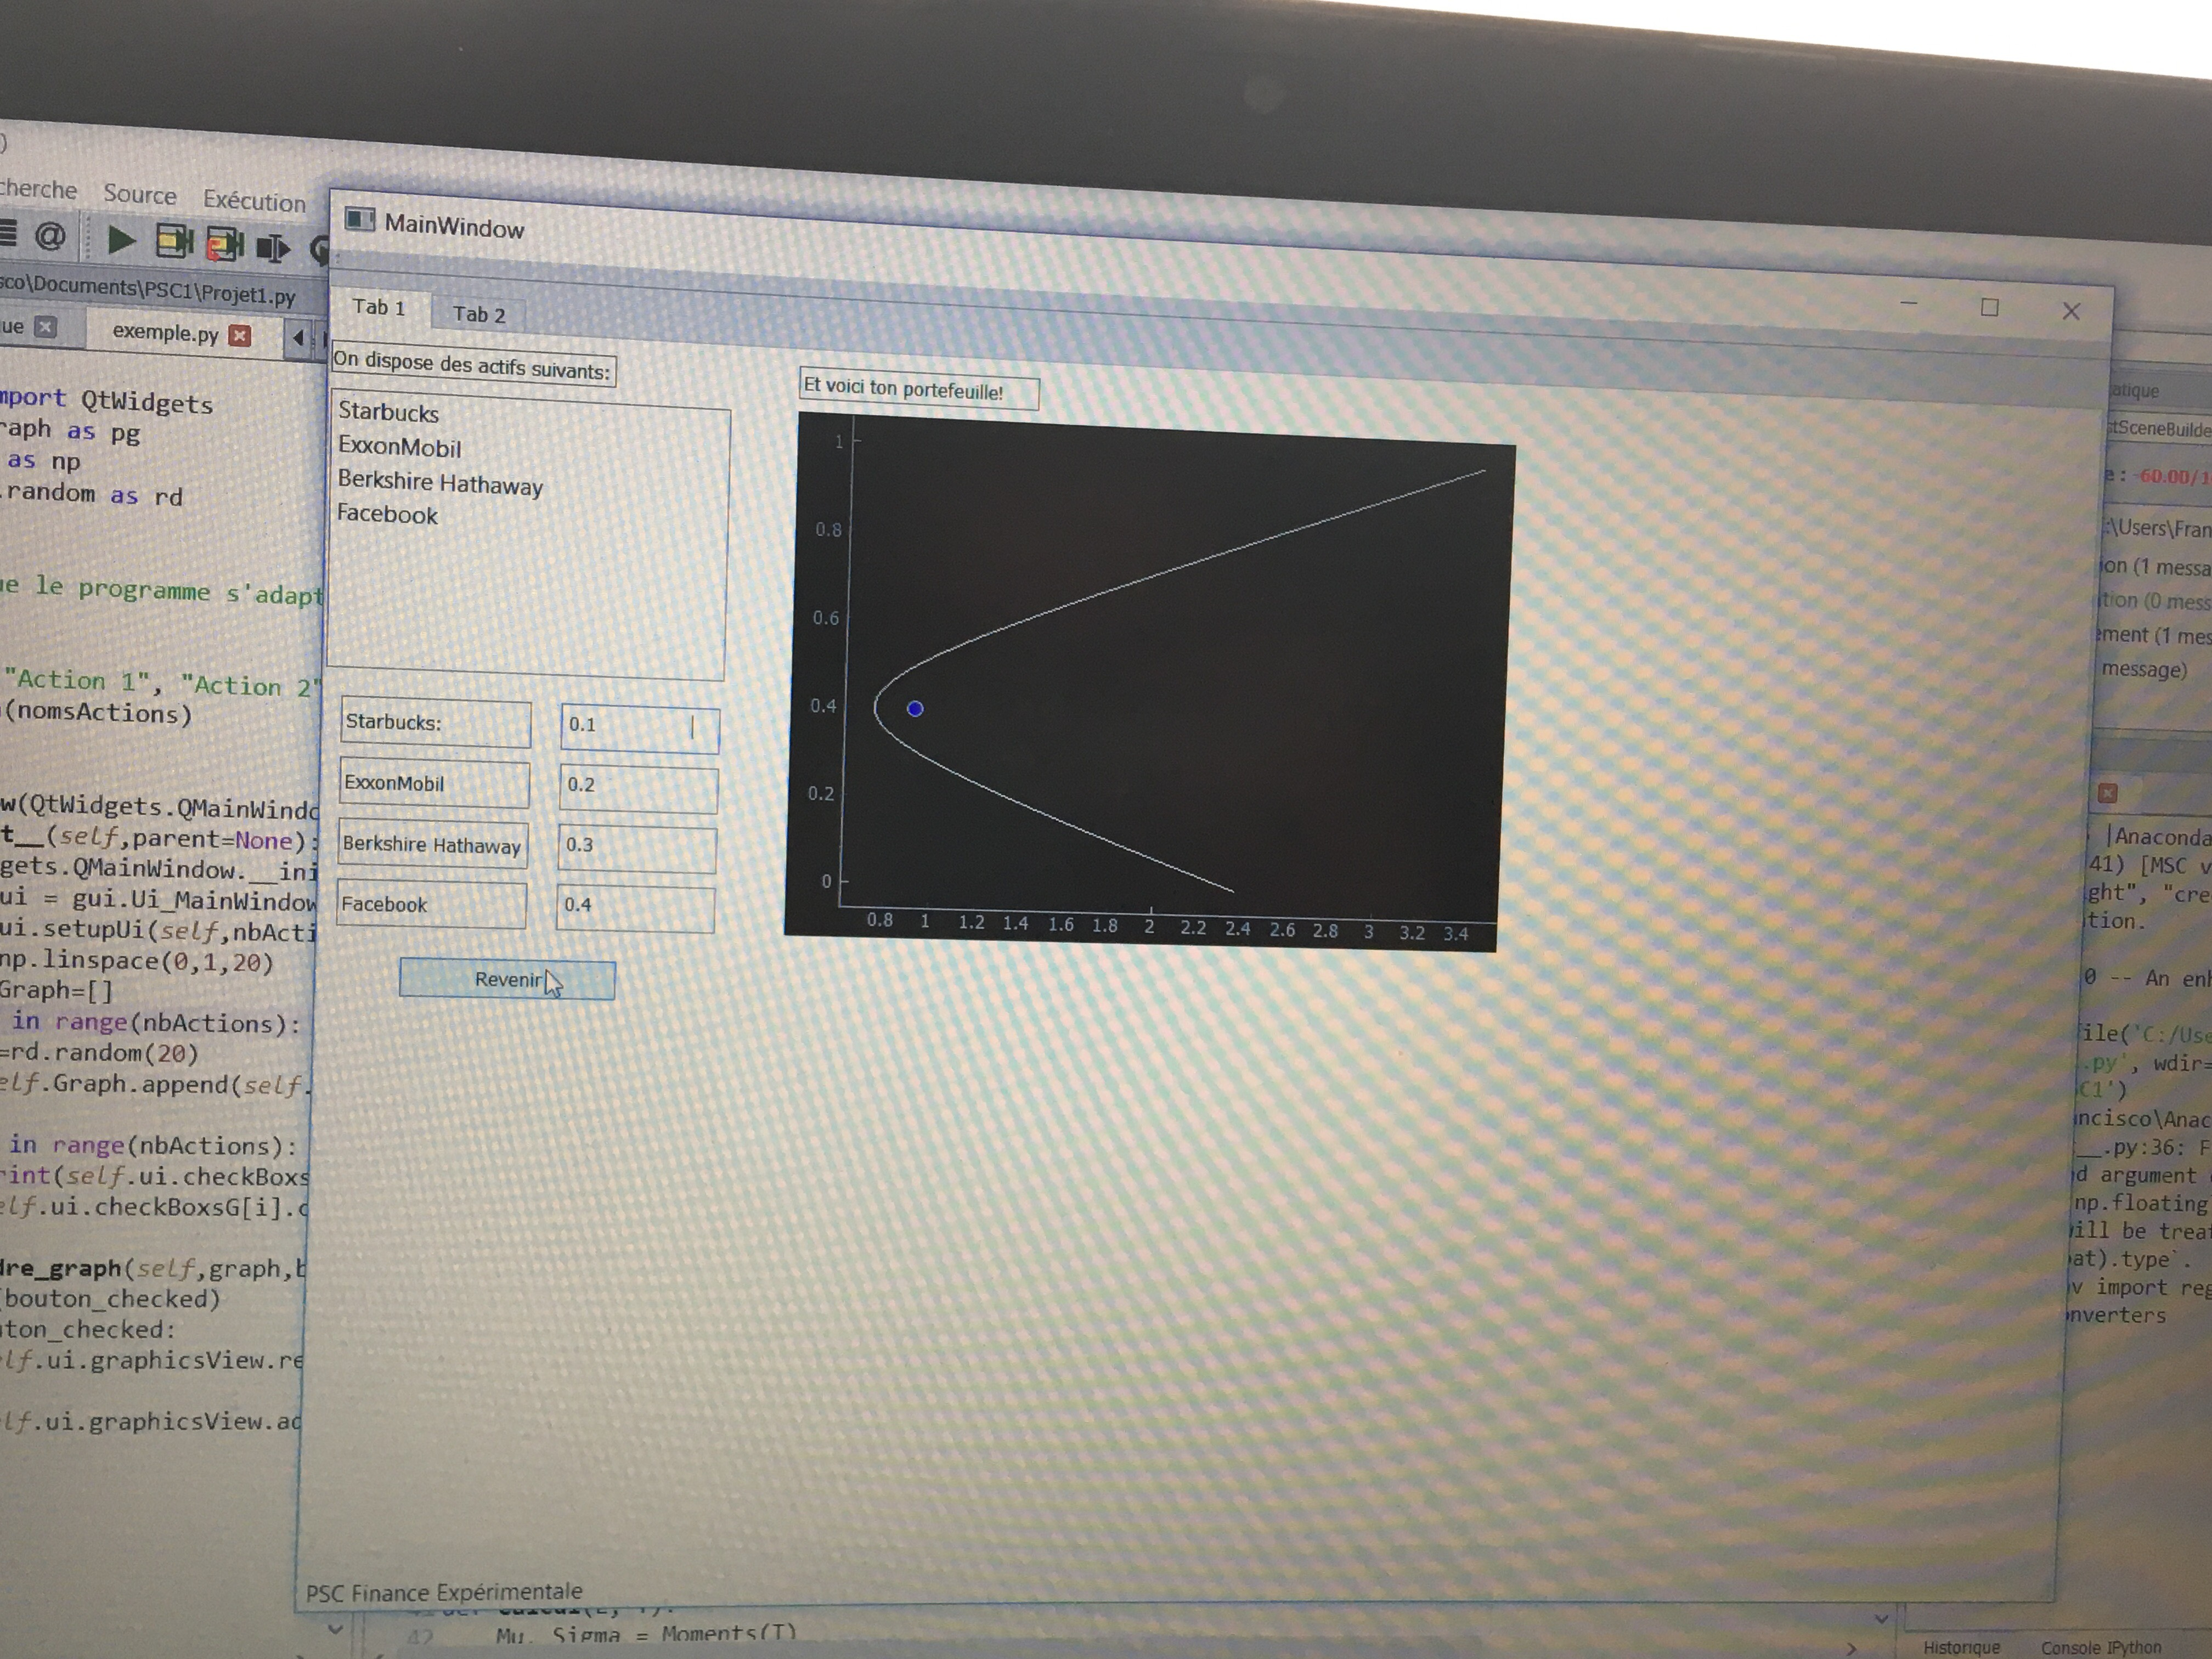
\includegraphics [width=8cm]{Im2.PNG}}
\caption{\label{} Frontière de Markovitz}
\end{figure} 

\end{document}